\chapter{Georeferencing}
\section{Georeferencing with point cloud}

It is possible to set session as ground truth.
Thus, optimization process (Pose GRAPH SLAM) will not change its poses.
Other sessions can be aligned against ground truth session by adding edges.

\begin{figure}[H]
	\centering
	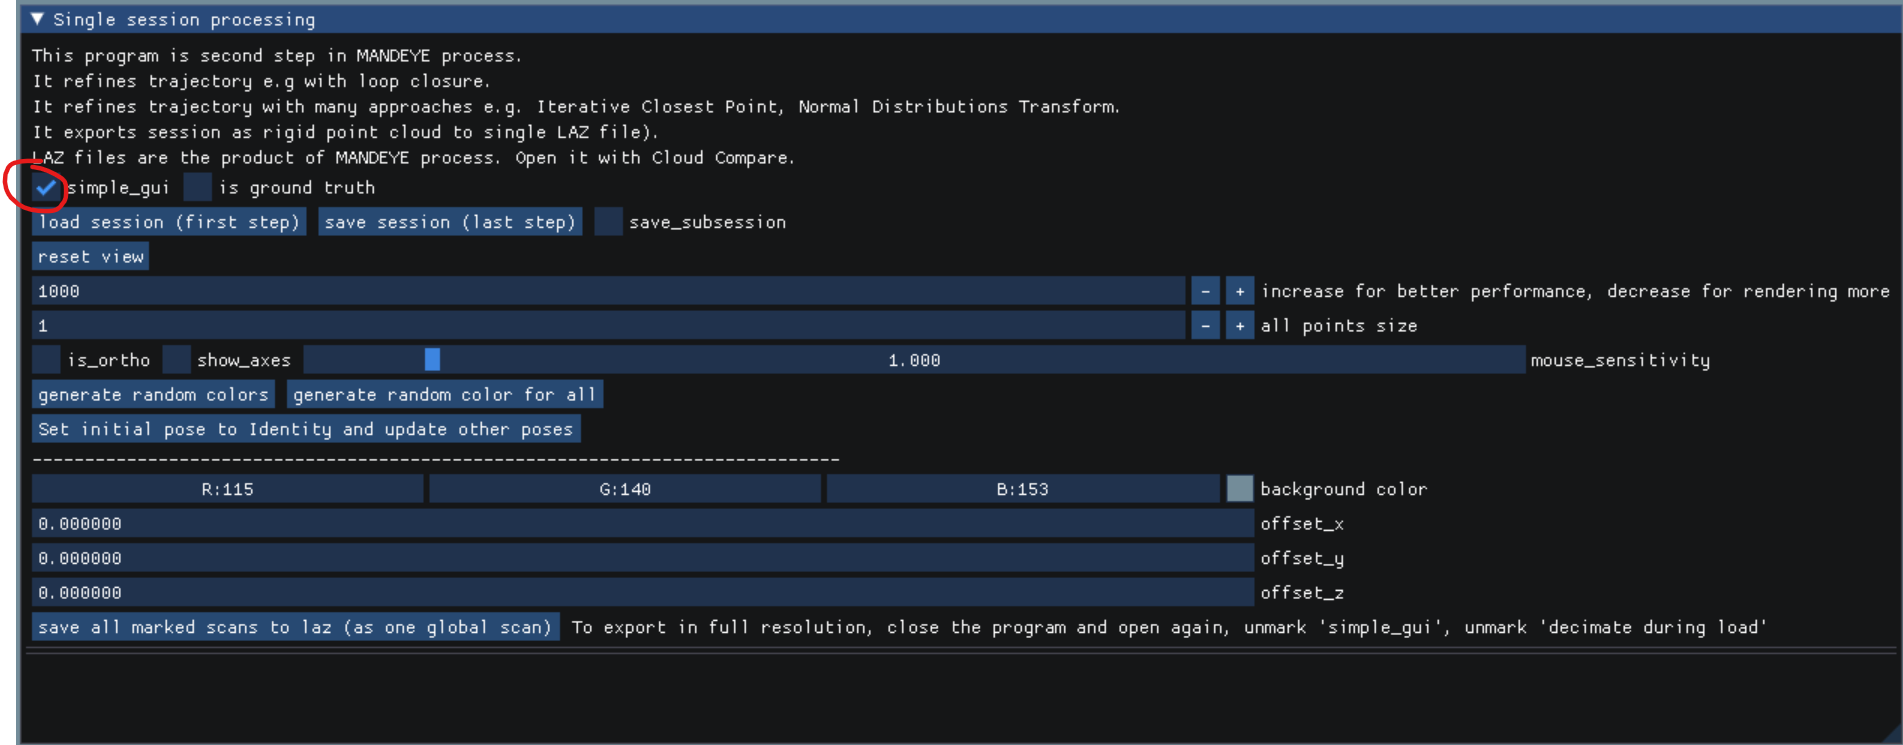
\includegraphics[width=\textwidth]{g1.png}
	\caption{Use multi view tls registration step2 program to open TLS files.}
	\label{fig:g1}
\end{figure}

\begin{figure}[H]
	\centering
	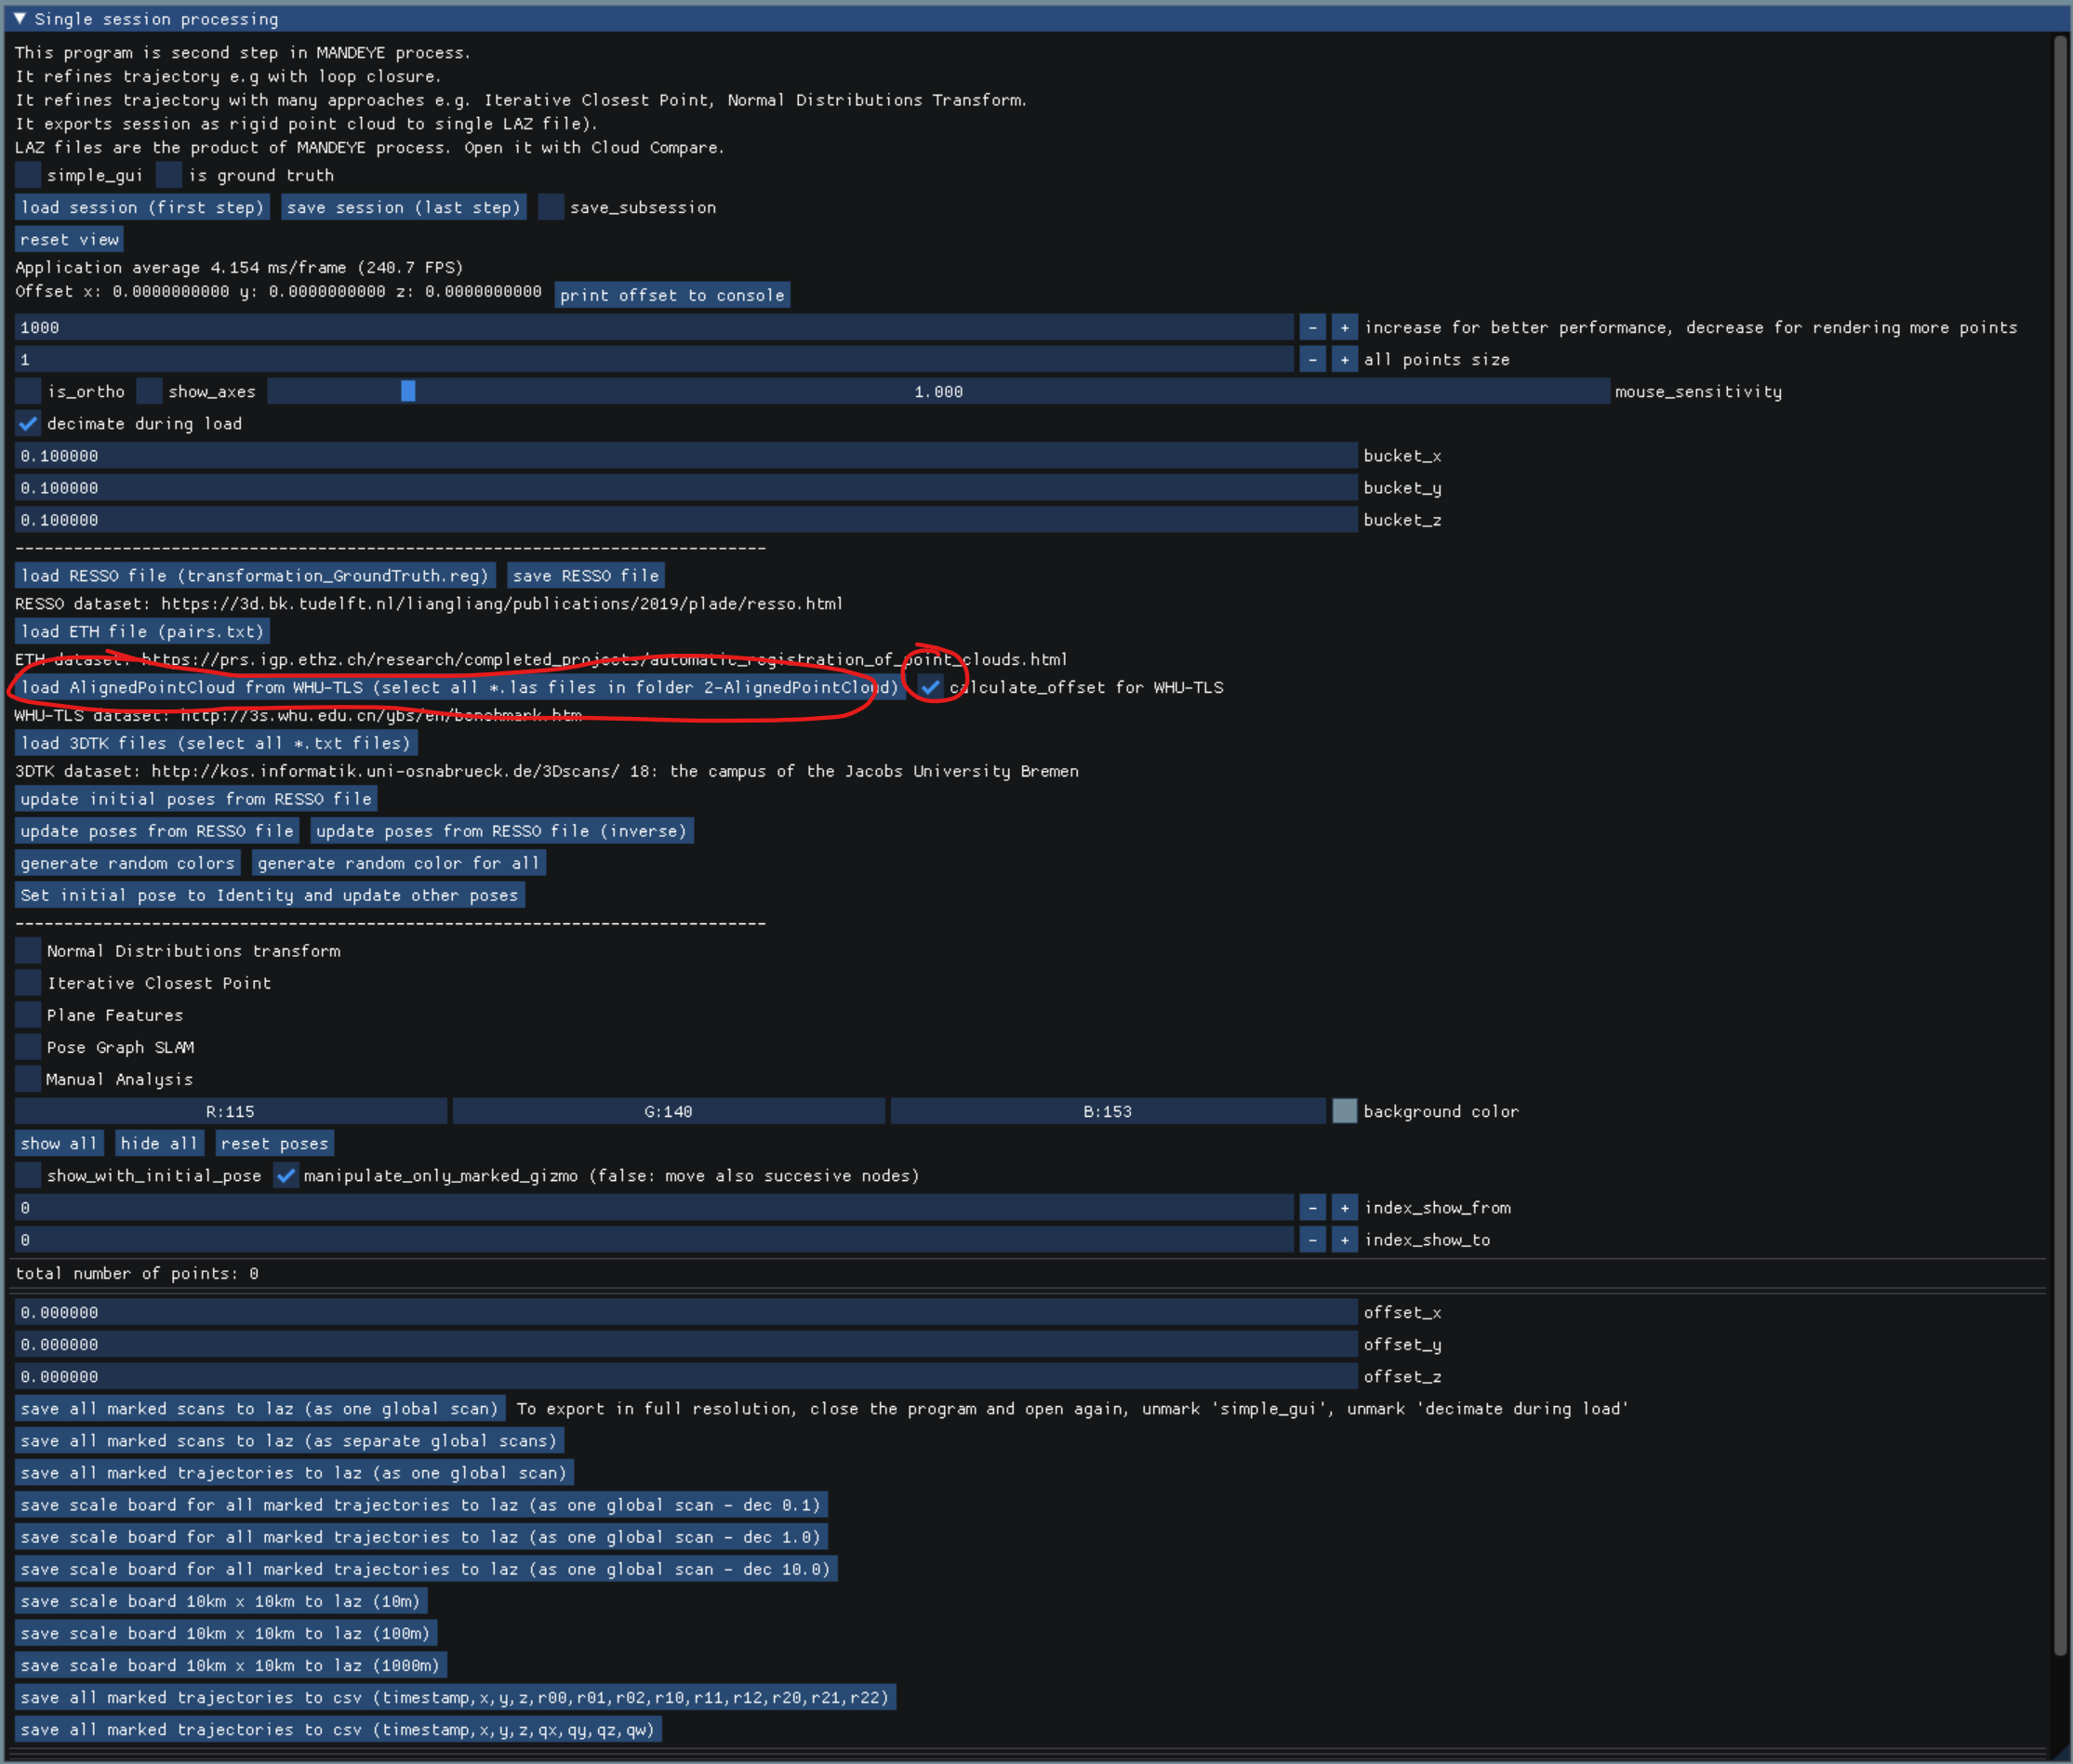
\includegraphics[width=\textwidth]{g2.png}
	\caption{Mark calculate offset for WHU-TLS, load AlignedPointCloud from WHU-TLS (select all *.las/laz files in folder)}
	\label{fig:g2}
\end{figure}

\begin{figure}[H]
	\centering
	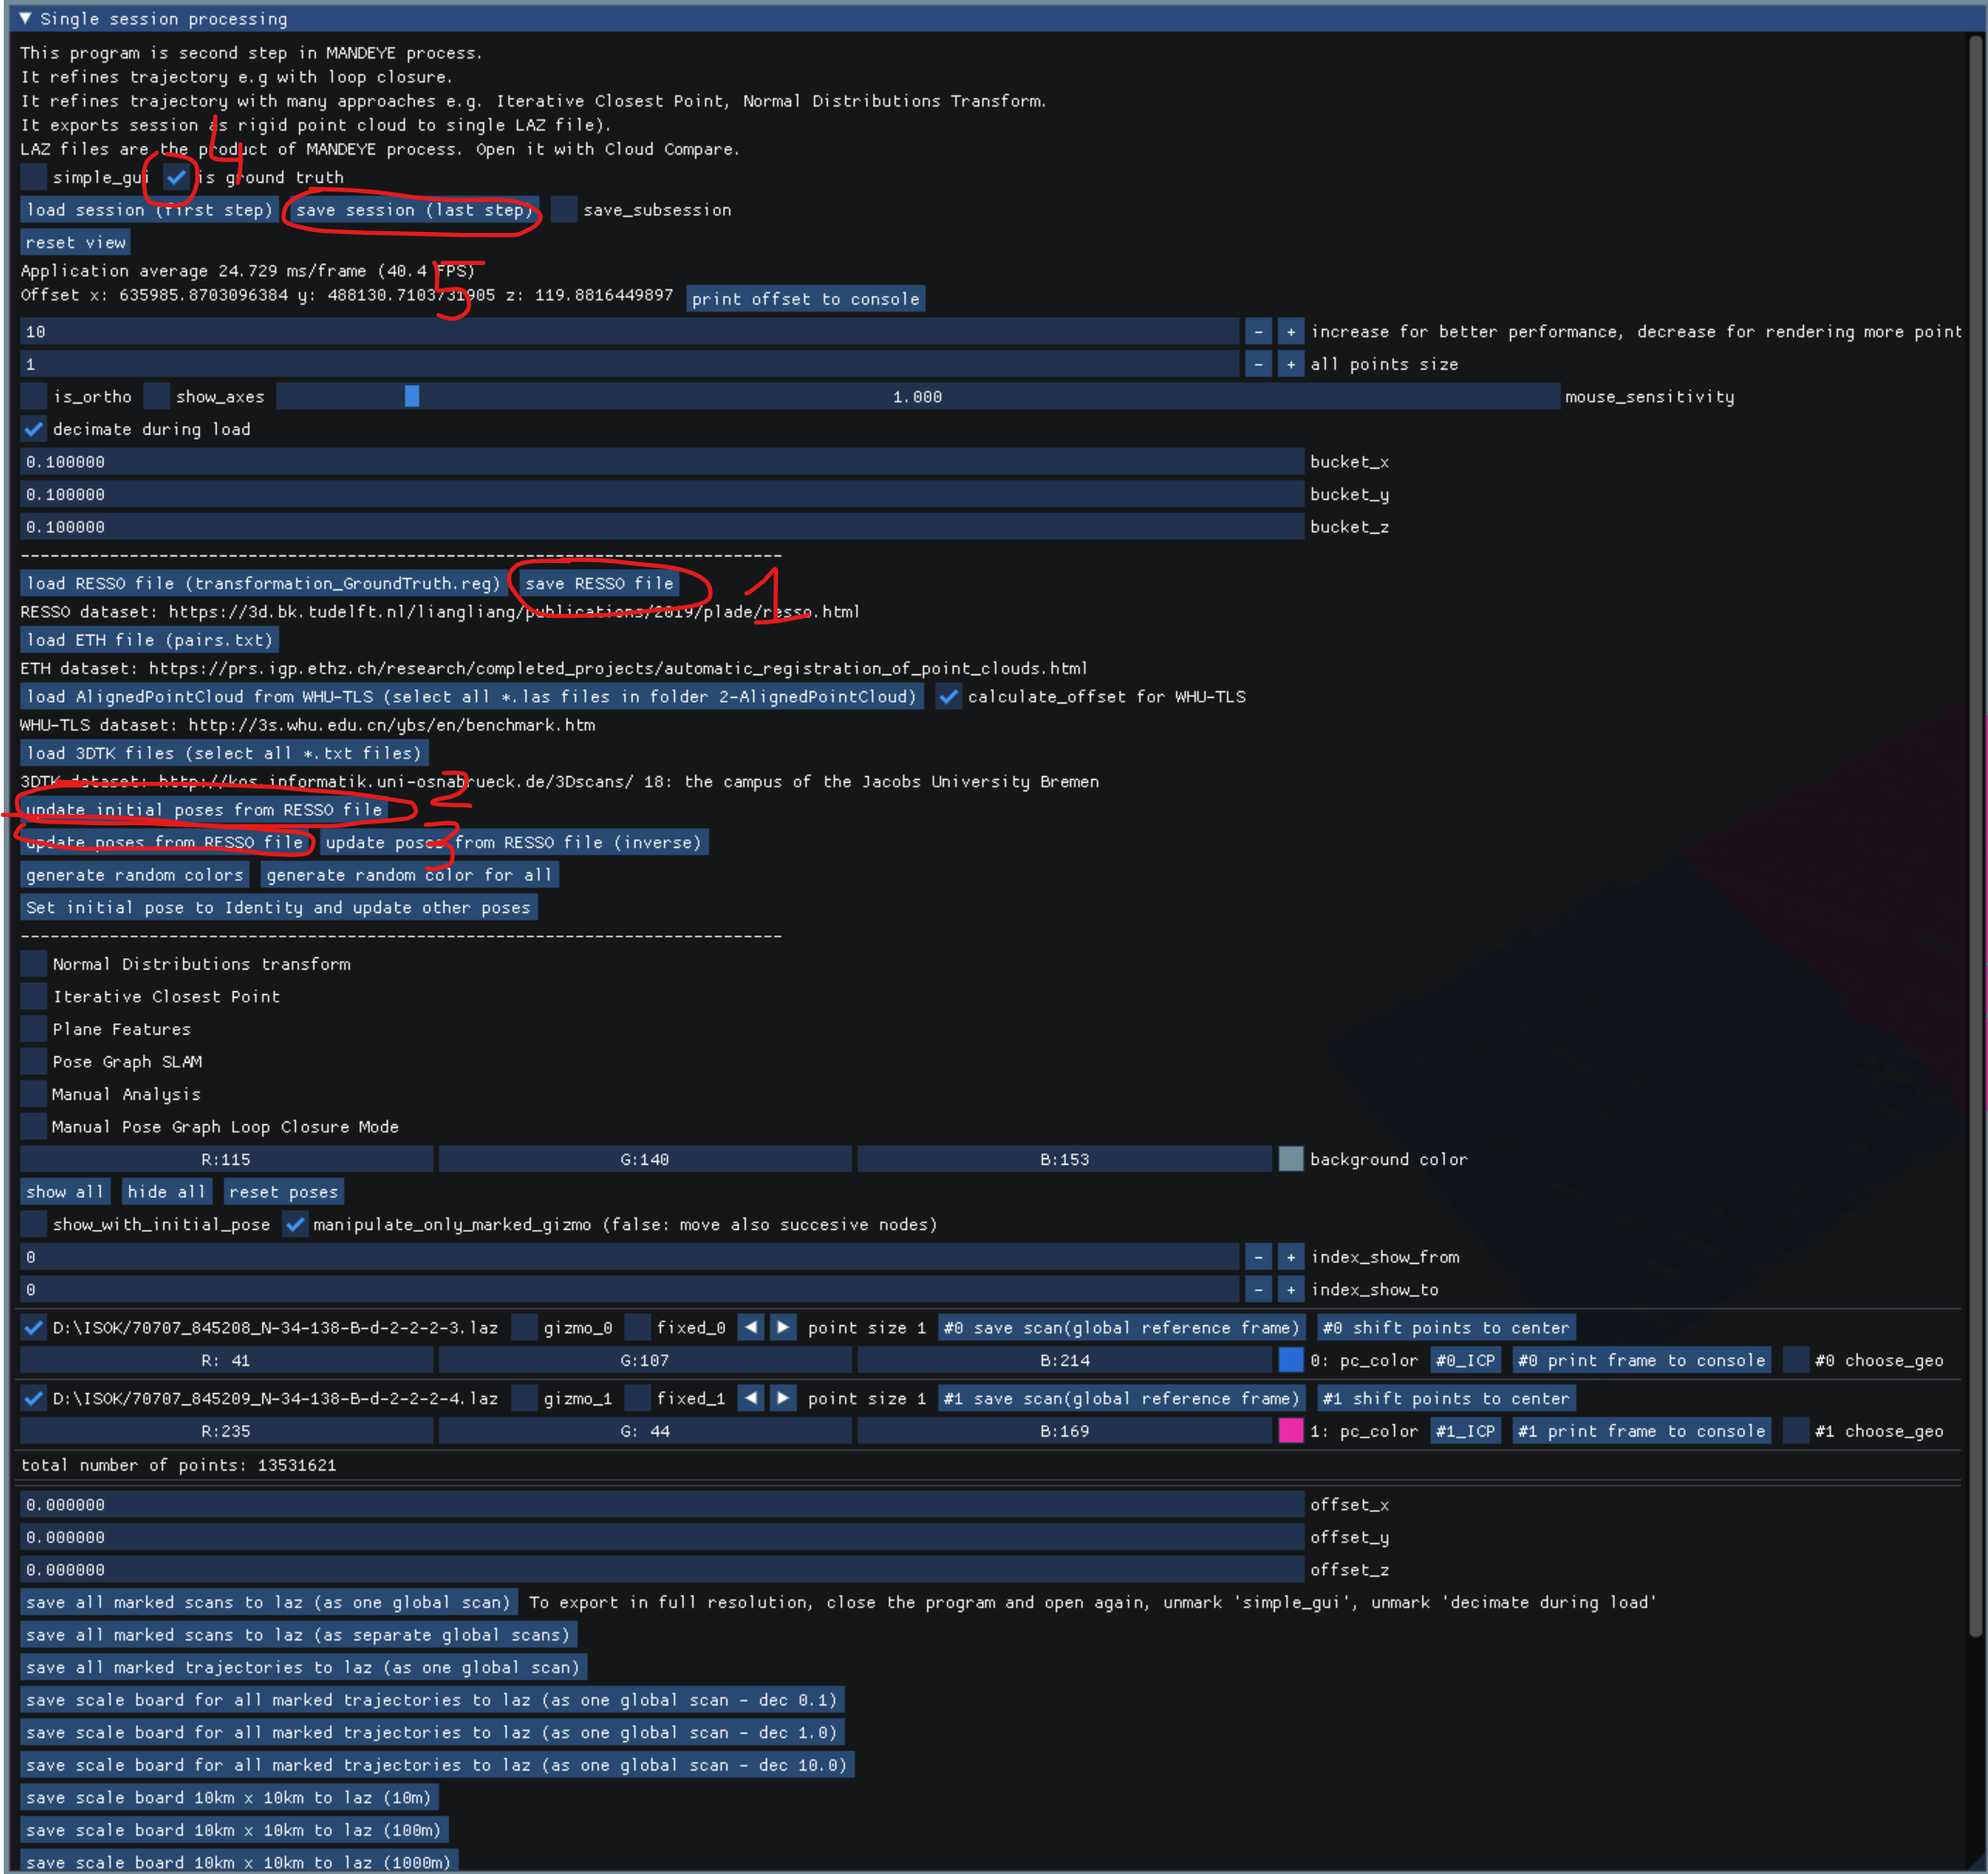
\includegraphics[width=\textwidth]{g3.png}
	\caption{1: save RESSO file, 2: update initial poses from RESSO file (select file from 1), 3: update poses from RESSO file (select file from 1), 4: set checkbox is ground truth, 5: save session.}
	\label{fig:g3}
\end{figure}

\section{Georeferencing with WGS84toCartesian}
\label{Georeferencing_with_WGS84toCartesian}
It uses \url{https://github.com/chrberger/WGS84toCartesian/tree/master} WGS84toCartesian.
It is a small and efficient library written in modern C++ library to convert WGS84 latitude/longitude positions to/from Cartesian positions using Mercator projection.
If You have MANDEYE with GNSS receiver, then it saves data in gnssXXXX.gnss files.
This is ASCII file with\\
---\\
timestamp lat lon alt hdop satelites-tracked height age time fix-quality\\
---\
\begin{figure}[H]
	\centering
	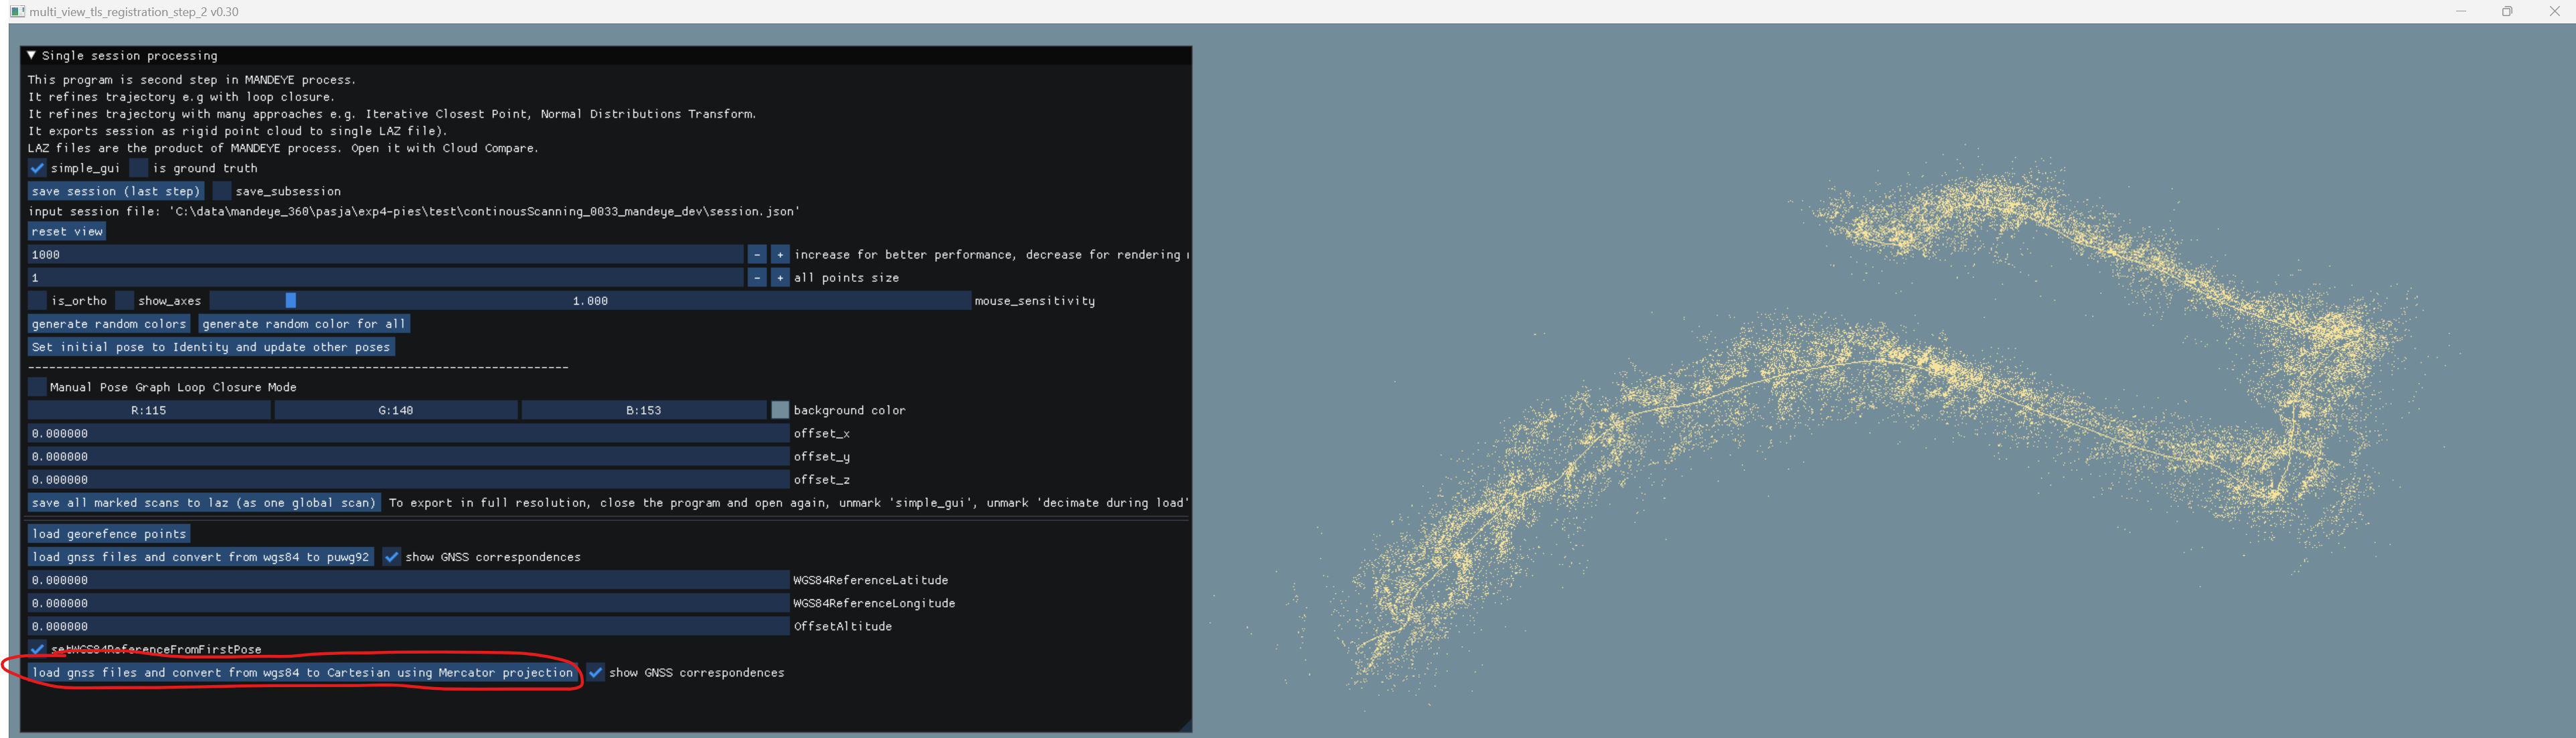
\includegraphics[width=\textwidth]{geo0.png}
	\caption{Georeferencing step 1: load gnss files and convert from wgs84 to Cartesian using Mercator projection.}
	\label{fig:geo0}
\end{figure}

\begin{figure}[H]
	\centering
	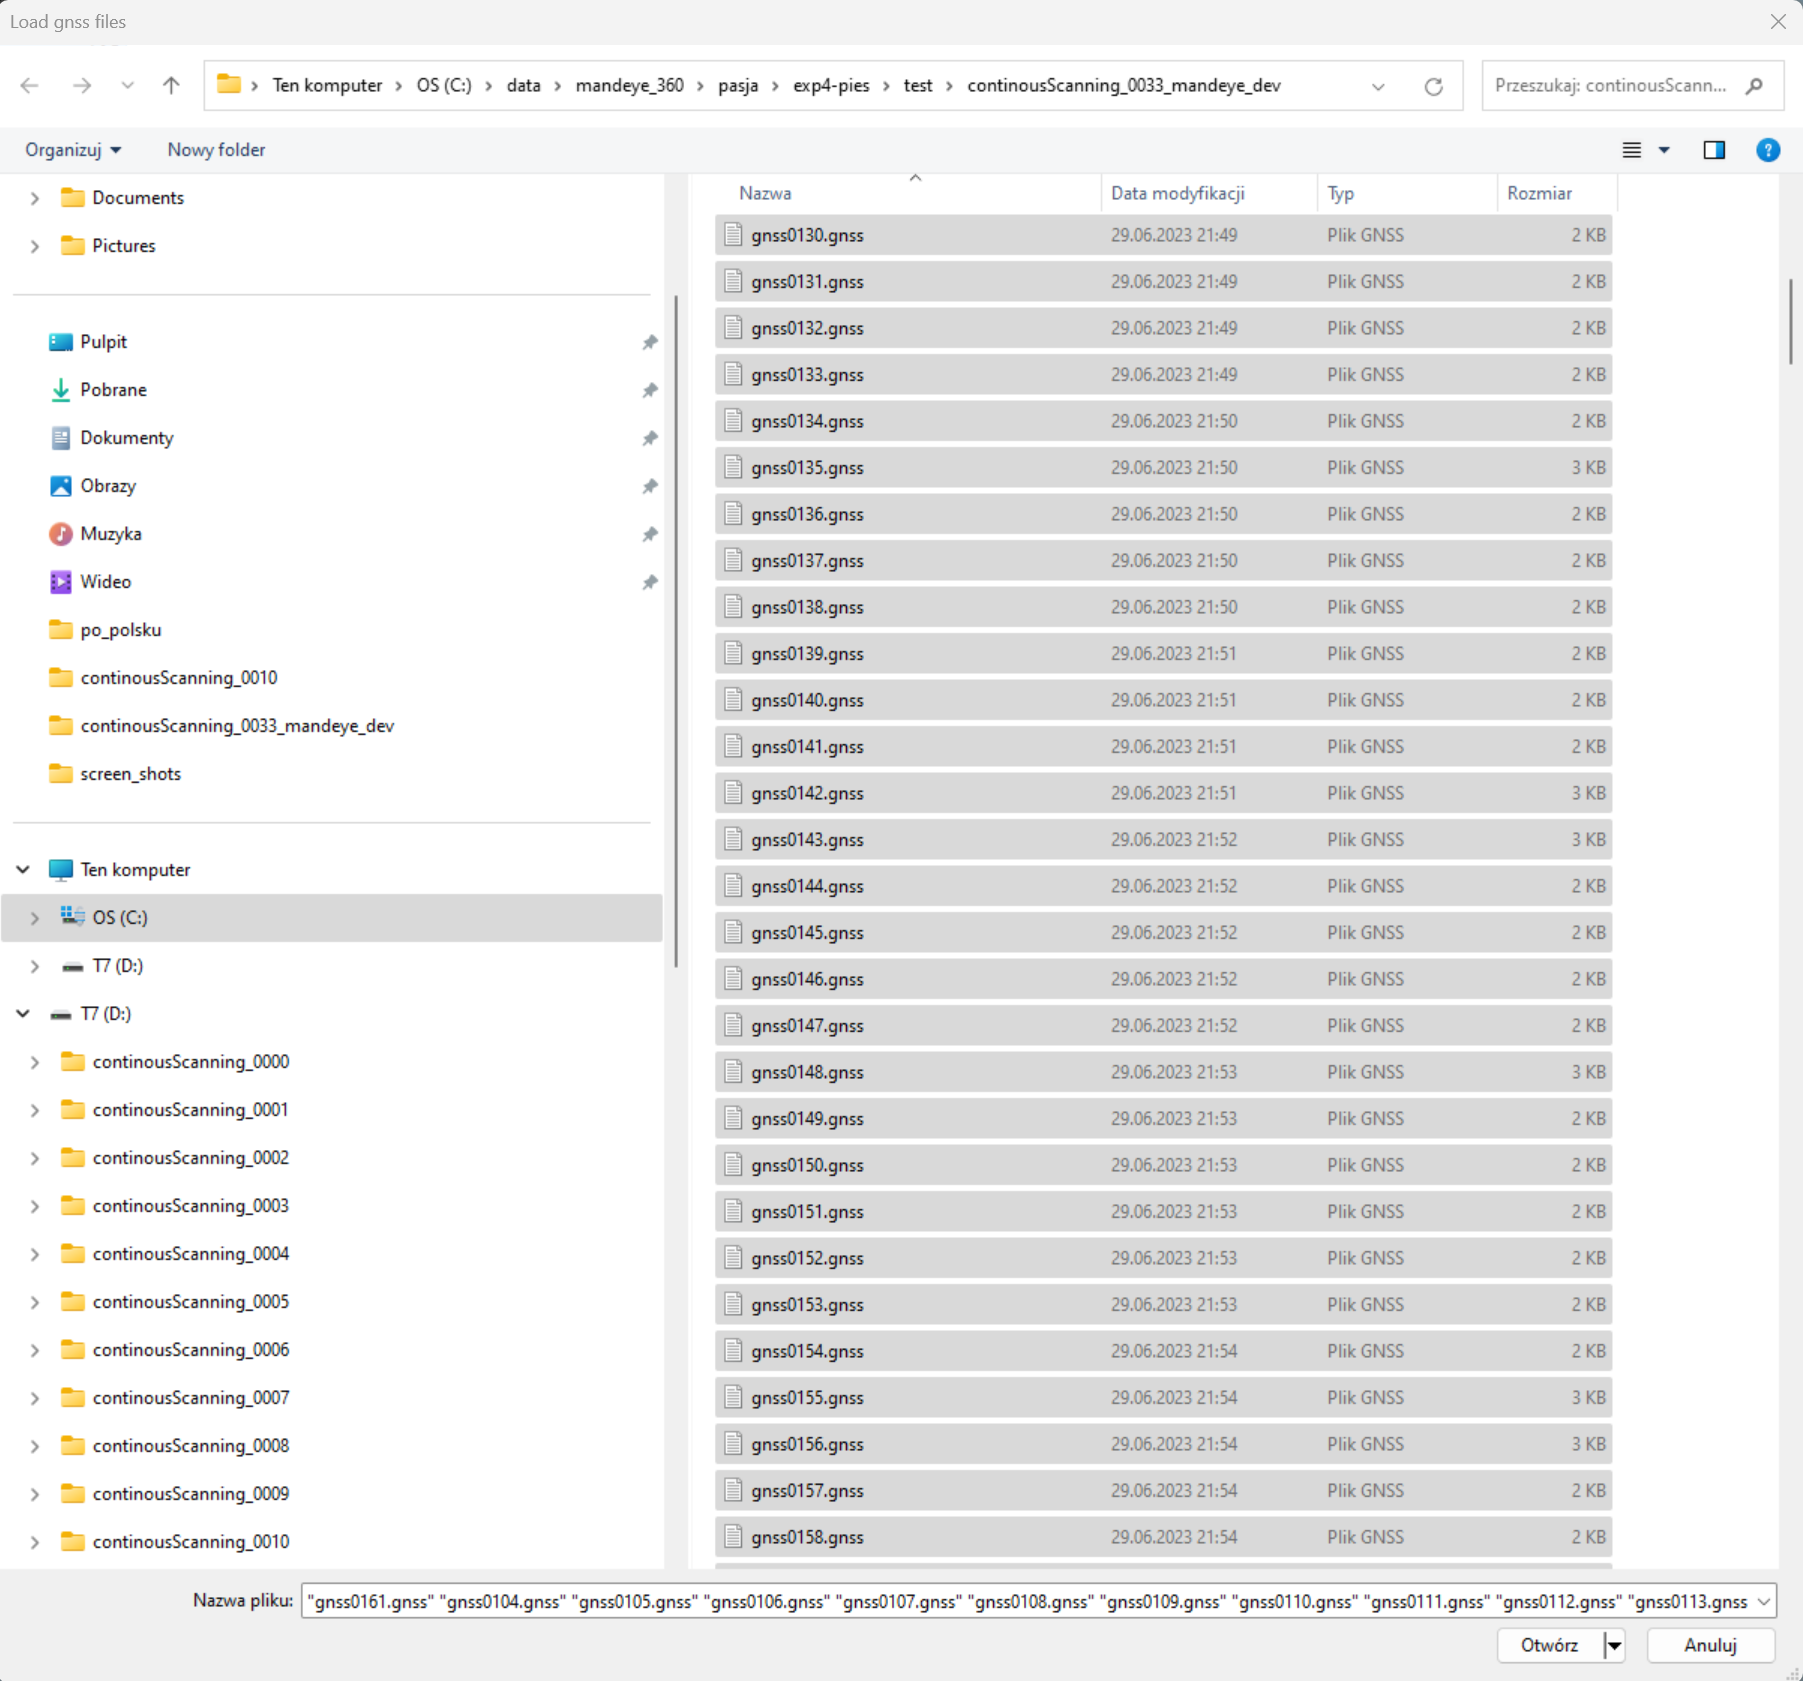
\includegraphics[width=\textwidth]{geo1.png}
	\caption{Georeferencing step 2: mark all gnss files and load.}
	\label{fig:geo1}
\end{figure}

\begin{figure}[H]
	\centering
	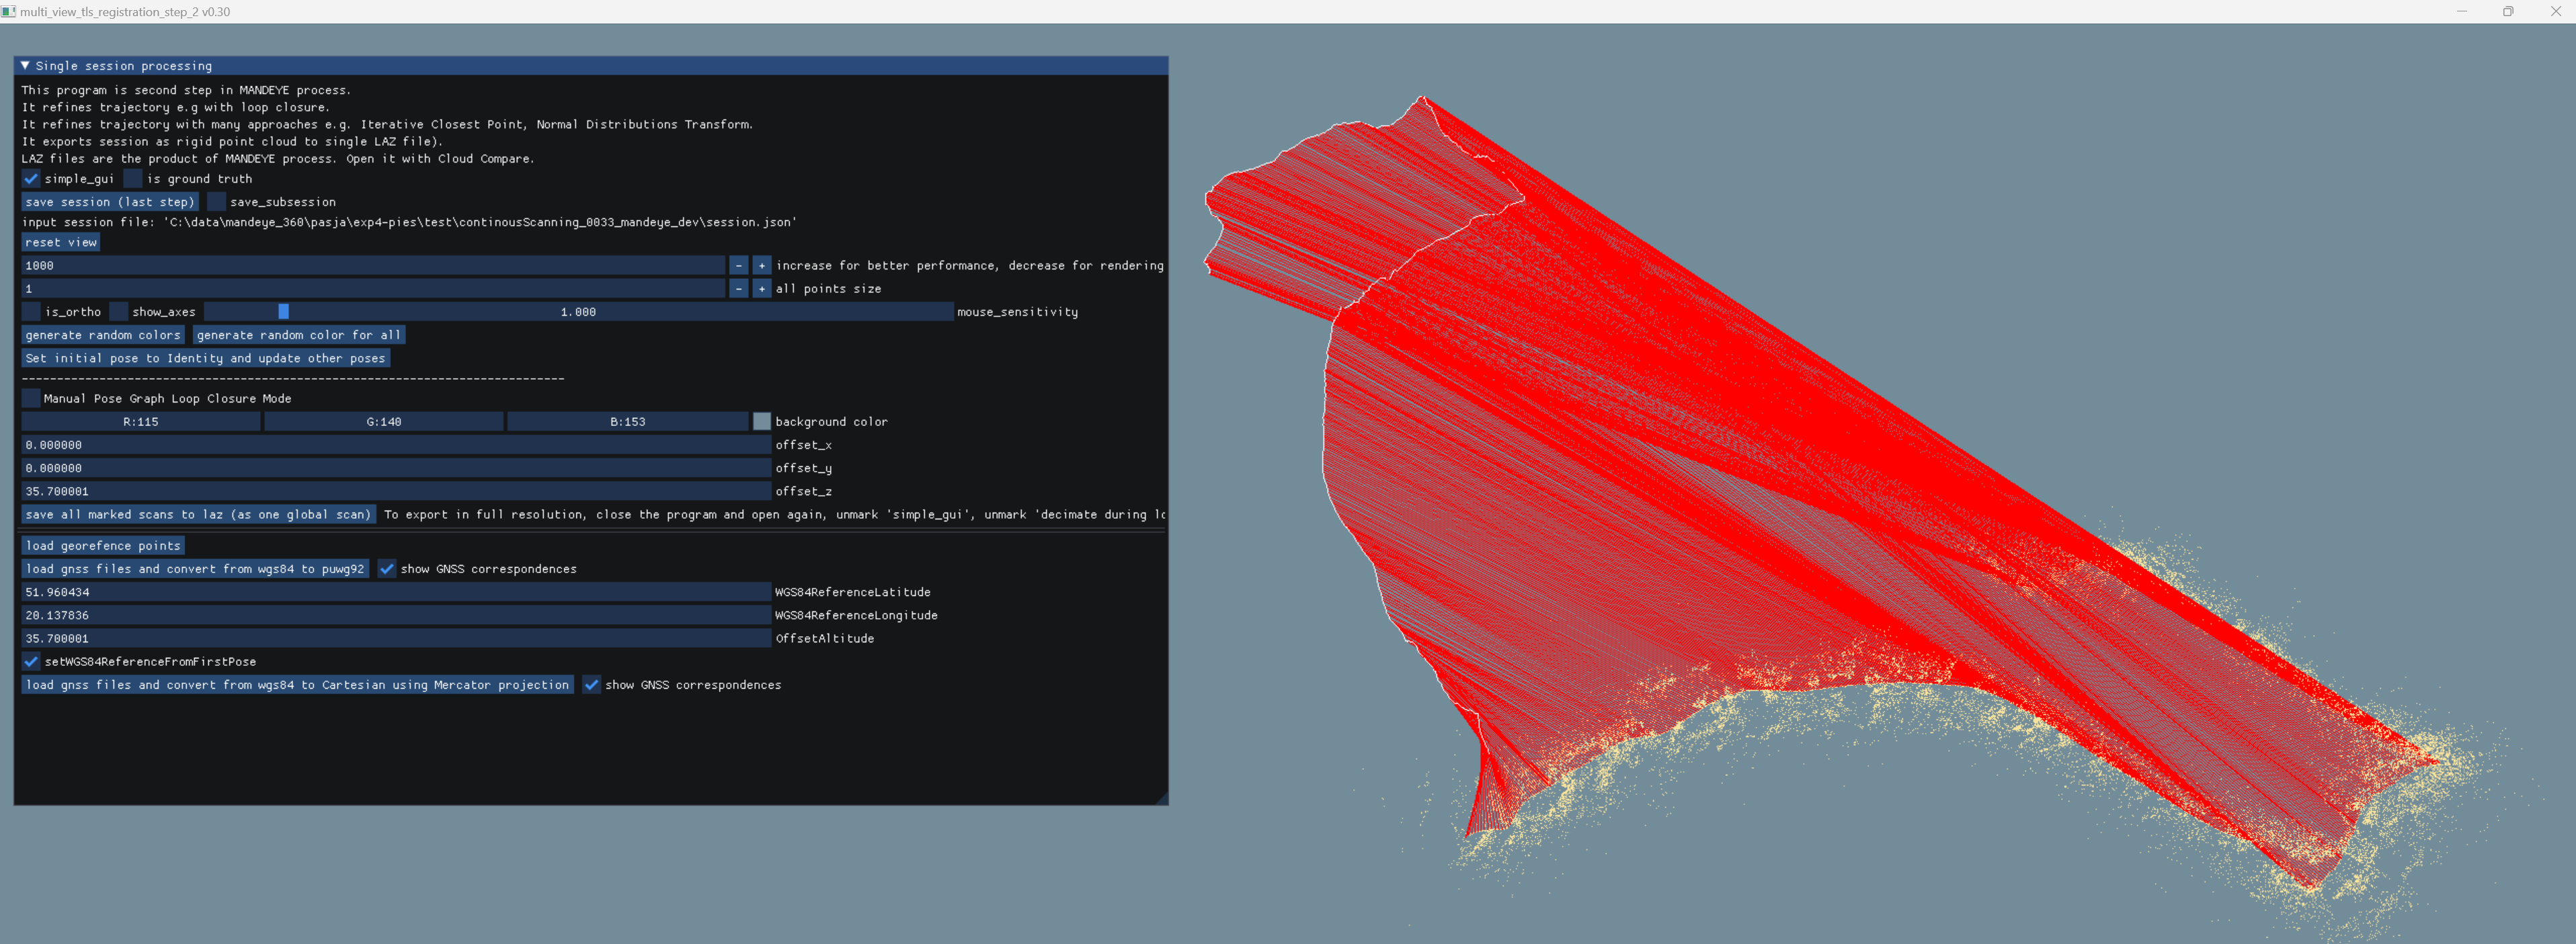
\includegraphics[width=\textwidth]{geo2.png}
	\caption{Georeferencing step 3: check/uncheck 'show GNSS correspondences' to see gnss-poses correspondences. Remark: You can use gizmo for manual initial trajectory to GNSS alignment.}
	\label{fig:geo2}
\end{figure}

\begin{figure}[H]
	\centering
	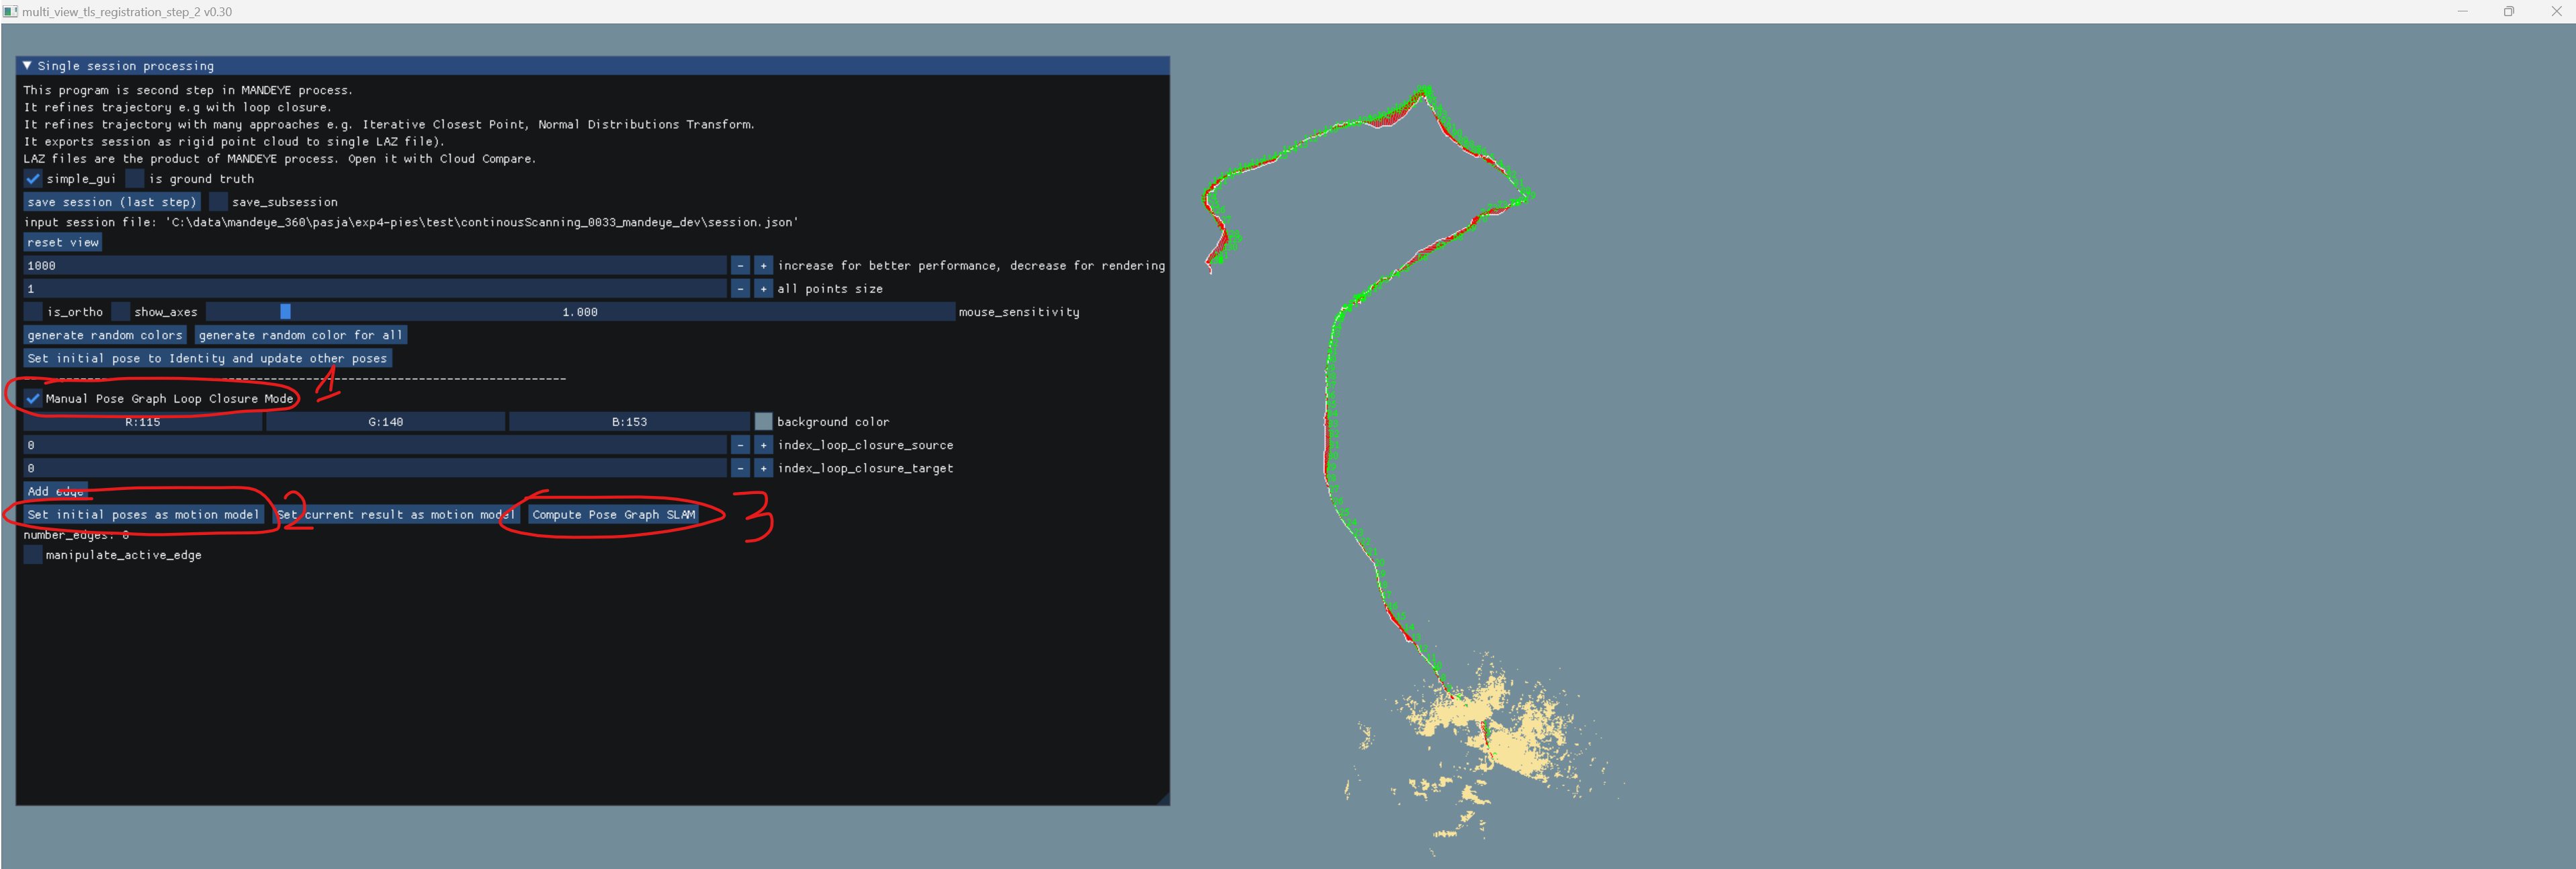
\includegraphics[width=\textwidth]{geo3.png}
	\caption{Georeferencing step 4: Check Manual Pose Graph Loop Closure Mode, then set initial poses as motion model, then Compute Pose Graph SLAM.}
	\label{fig:geo3}
\end{figure}
\pagebreak

\textbf{Below is an example of how to download and create ground truth data from exemplary ALS data (free polish ALS data available as part of ISOK: \url{http://www.gugik.gov.pl/projekty/isok/produkty}) with scans prepared through HDMapping software.}
Figures from \ref{fig:34} to \ref{fig:38} serve only as an example of how the process of gathering and preparing ALS data may look like.

To download ALS data Geoportal site will be used - \url{https://www.geoportal.gov.pl}.

\begin{figure}[H]
	\centering
	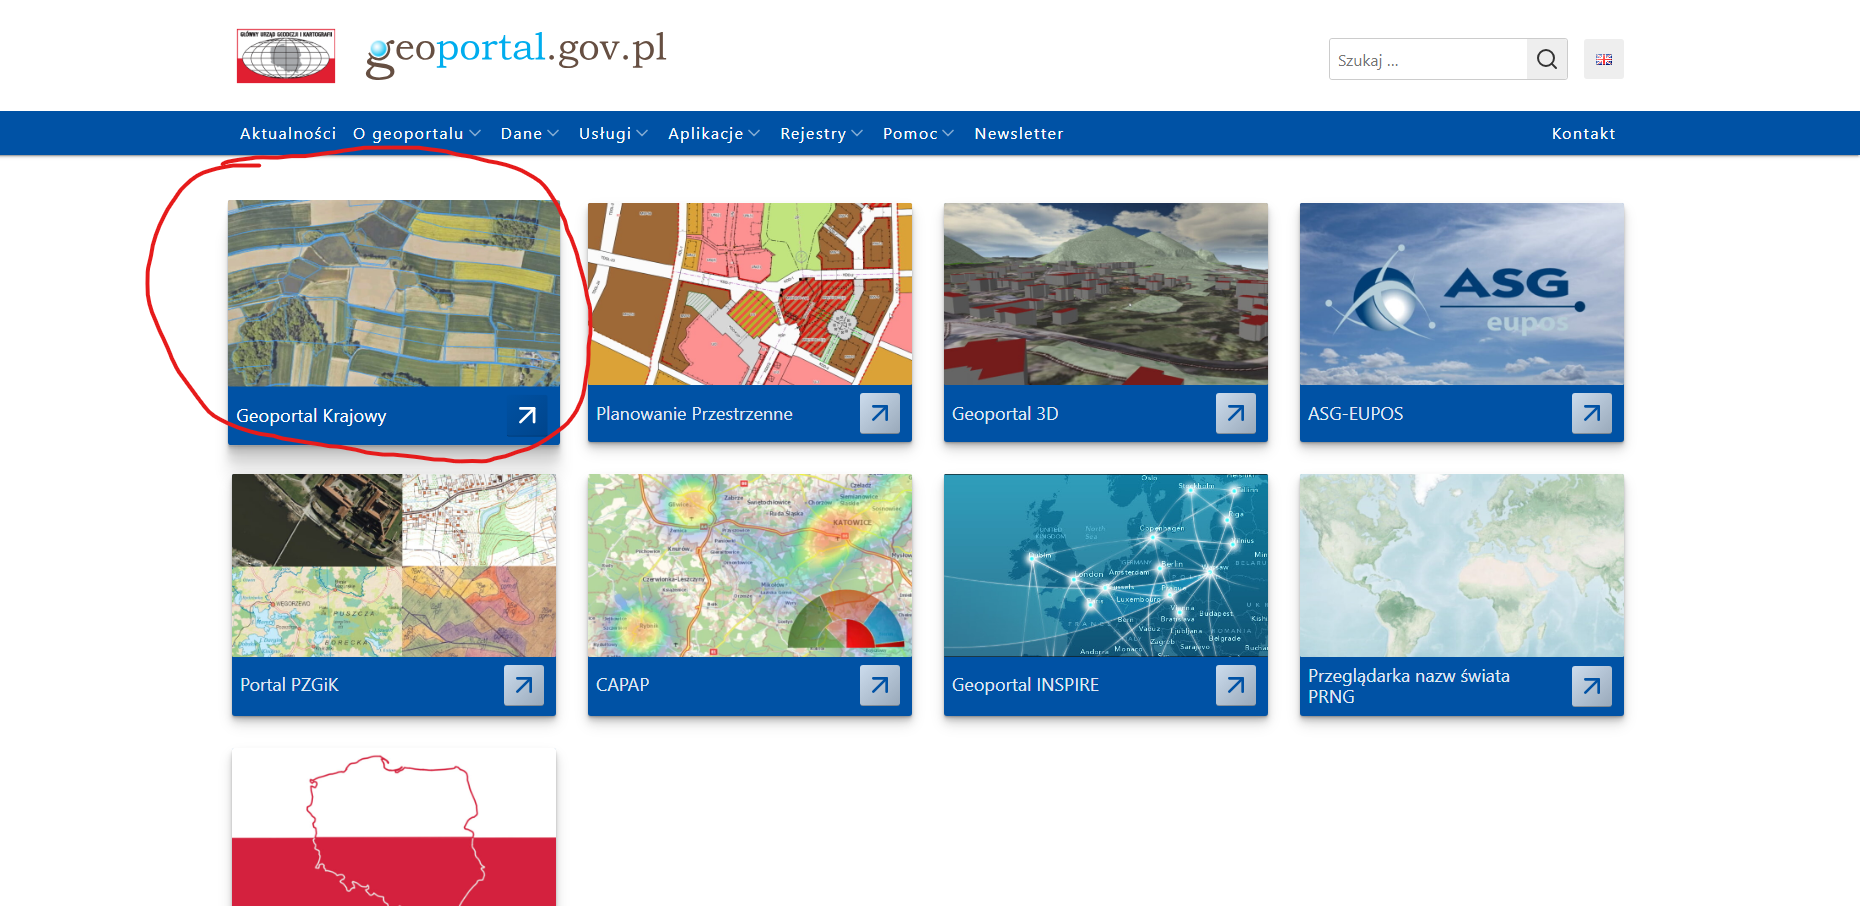
\includegraphics[width=\textwidth]{ISOK1.png}
	\caption{After \url{https://www.geoportal.gov.pl} site is loaded choose Geoportal krajowy tab.}
	\label{fig:34}
\end{figure}

\begin{figure}[H]
	\centering
	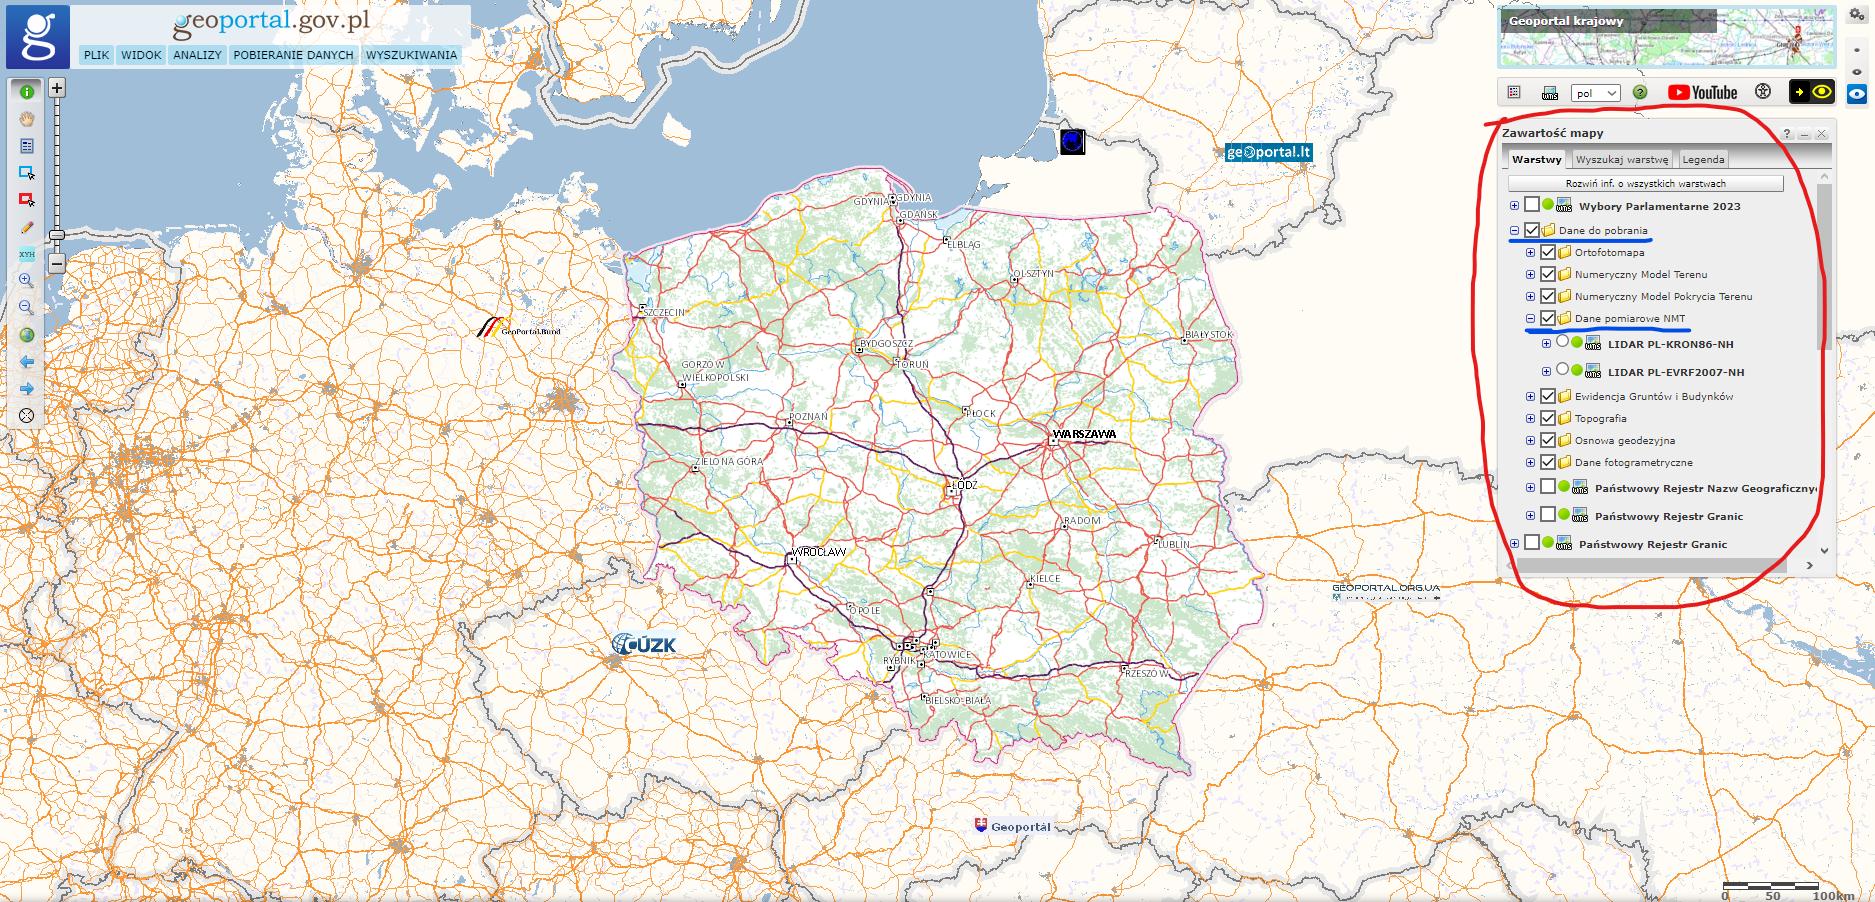
\includegraphics[width=\textwidth]{ISOK2.png}
	\caption{After Geoportal has loaded, on the right side of the screen select Dane do pobrania, then Dane pomiarowe NMT, where 2 options are possible.}
	\label{fig:35}
\end{figure}

\begin{figure}[H]
	\centering
	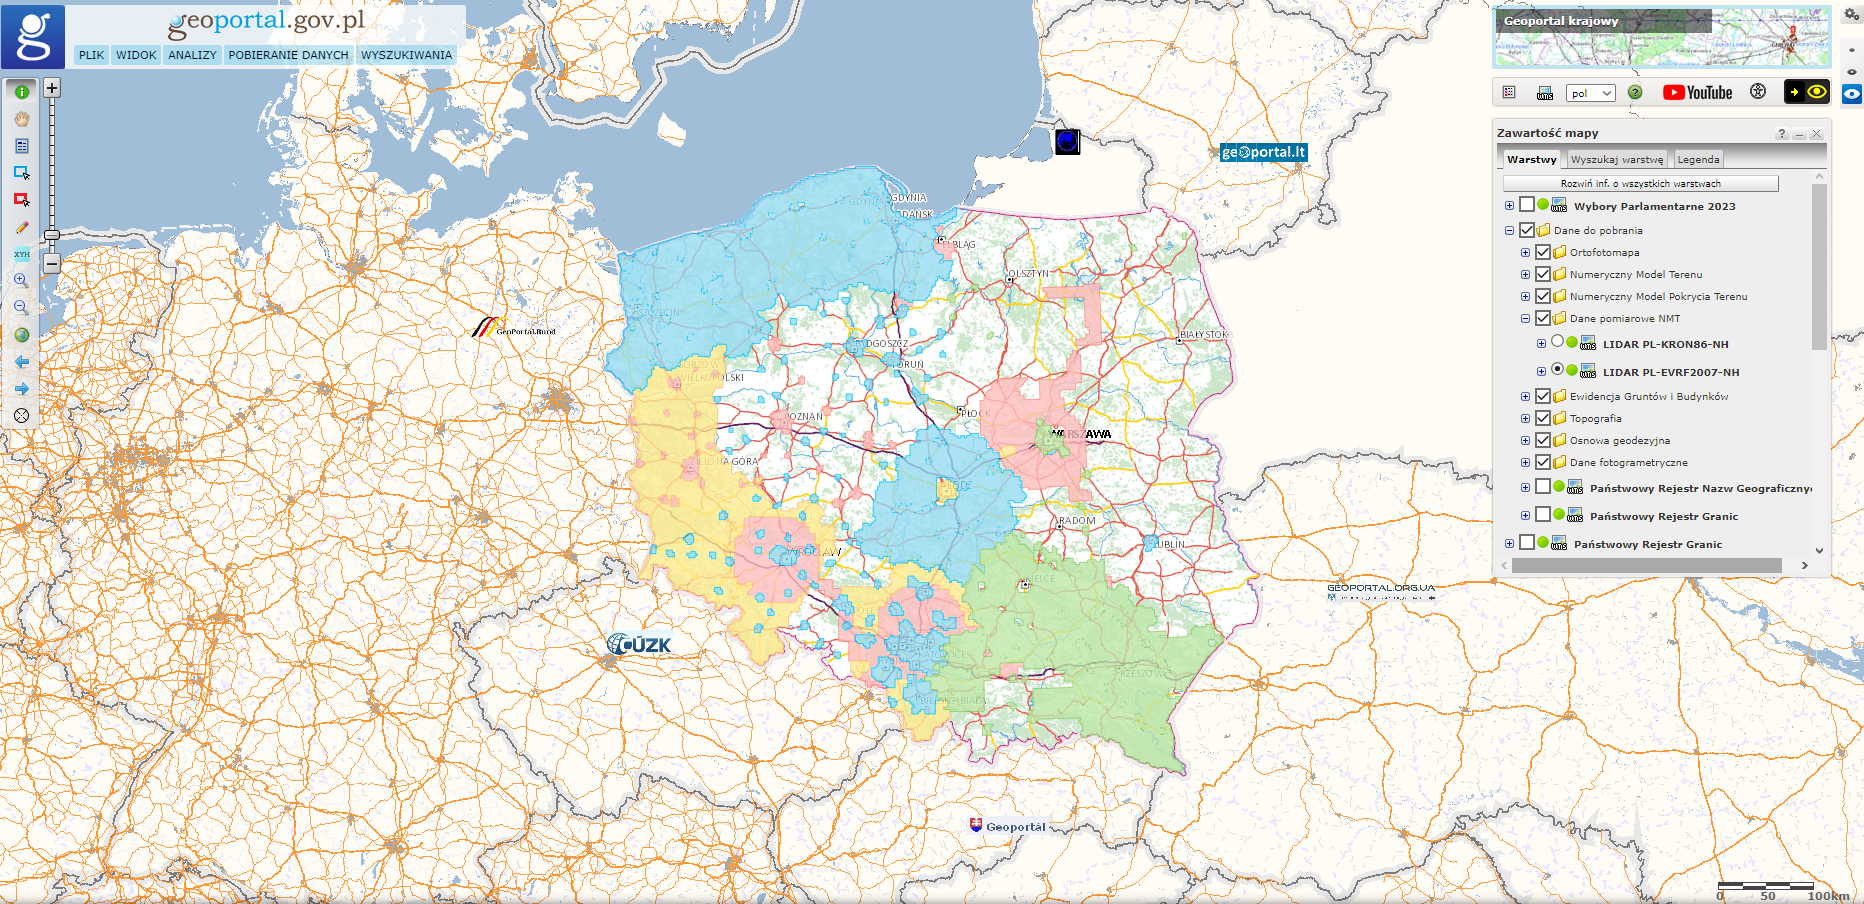
\includegraphics[width=\textwidth]{ISOK3.png}
	\caption{Whenever it is possible EVRF LIDAR version should be chosen over KRON36 version, as the former is more current than the latter. As can be seen on the screen there are parts without EVRF version and in such cases KRON86 is the only option.}
	\label{fig:36}
\end{figure}

\begin{figure}[H]
	\centering
	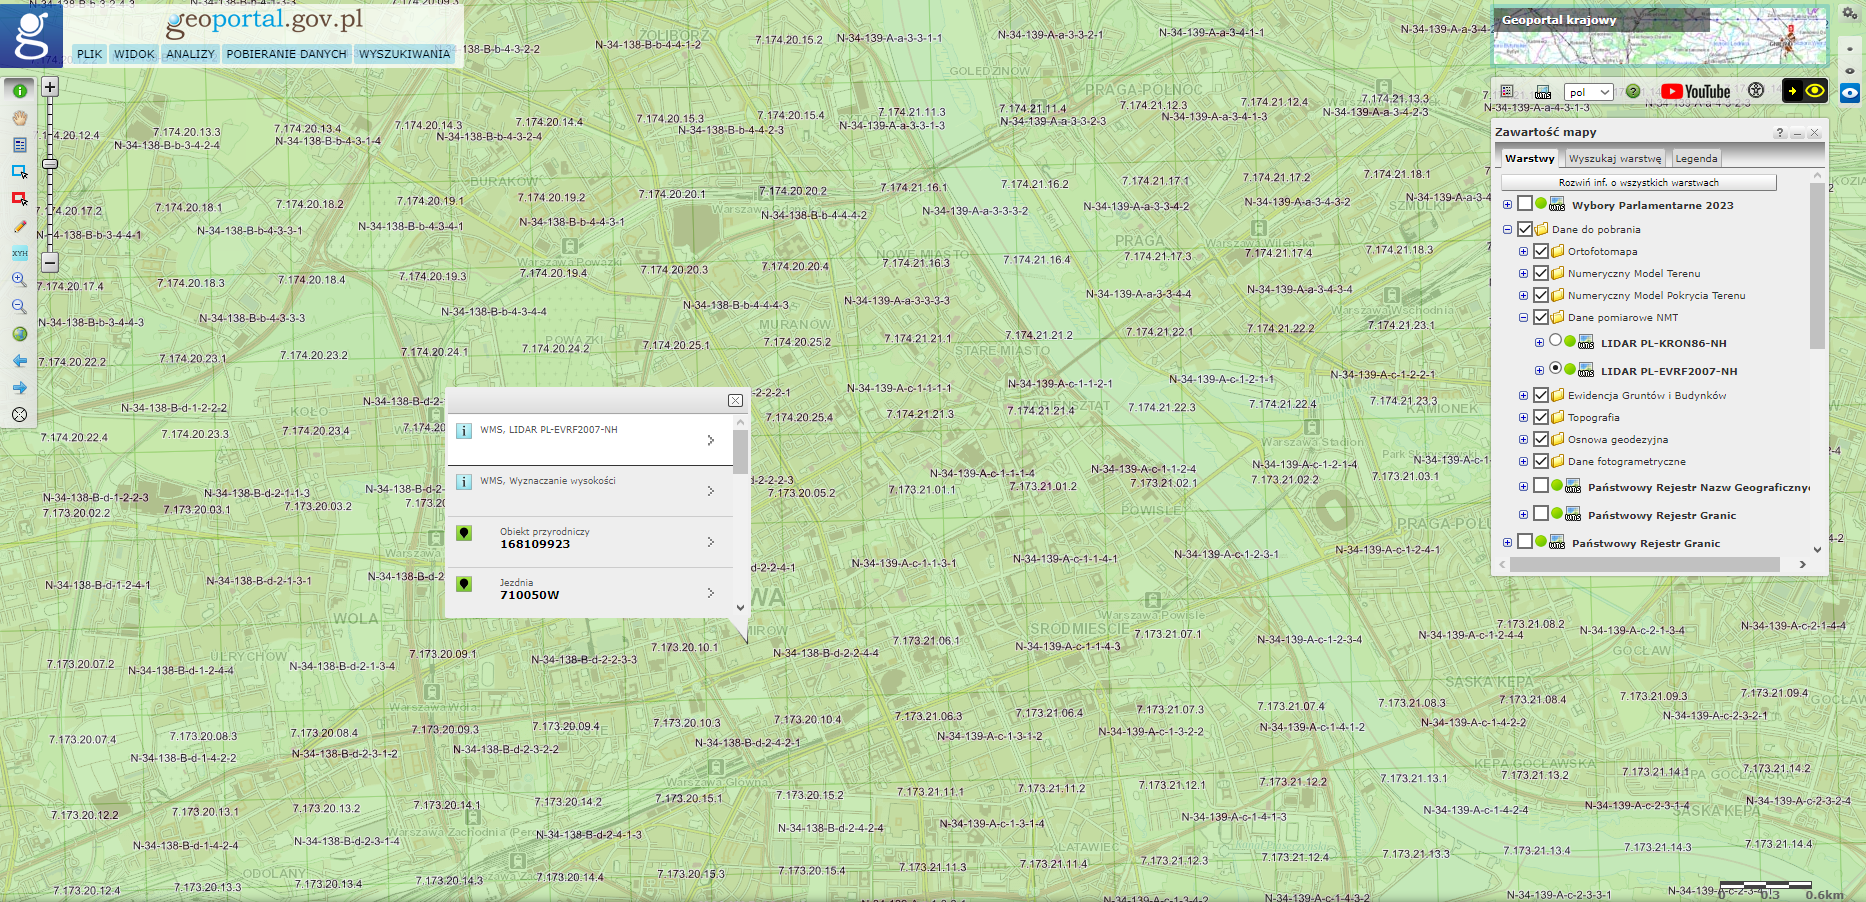
\includegraphics[width=\textwidth]{ISOK4.png}
	\caption{When LIDAR has been chosen zoom in to the map until tiles are seen. To download simply click on the tile with left mouse button and choose WMS, LIDAR.}
	\label{fig:37}
\end{figure}

\begin{figure}[H]
	\centering
	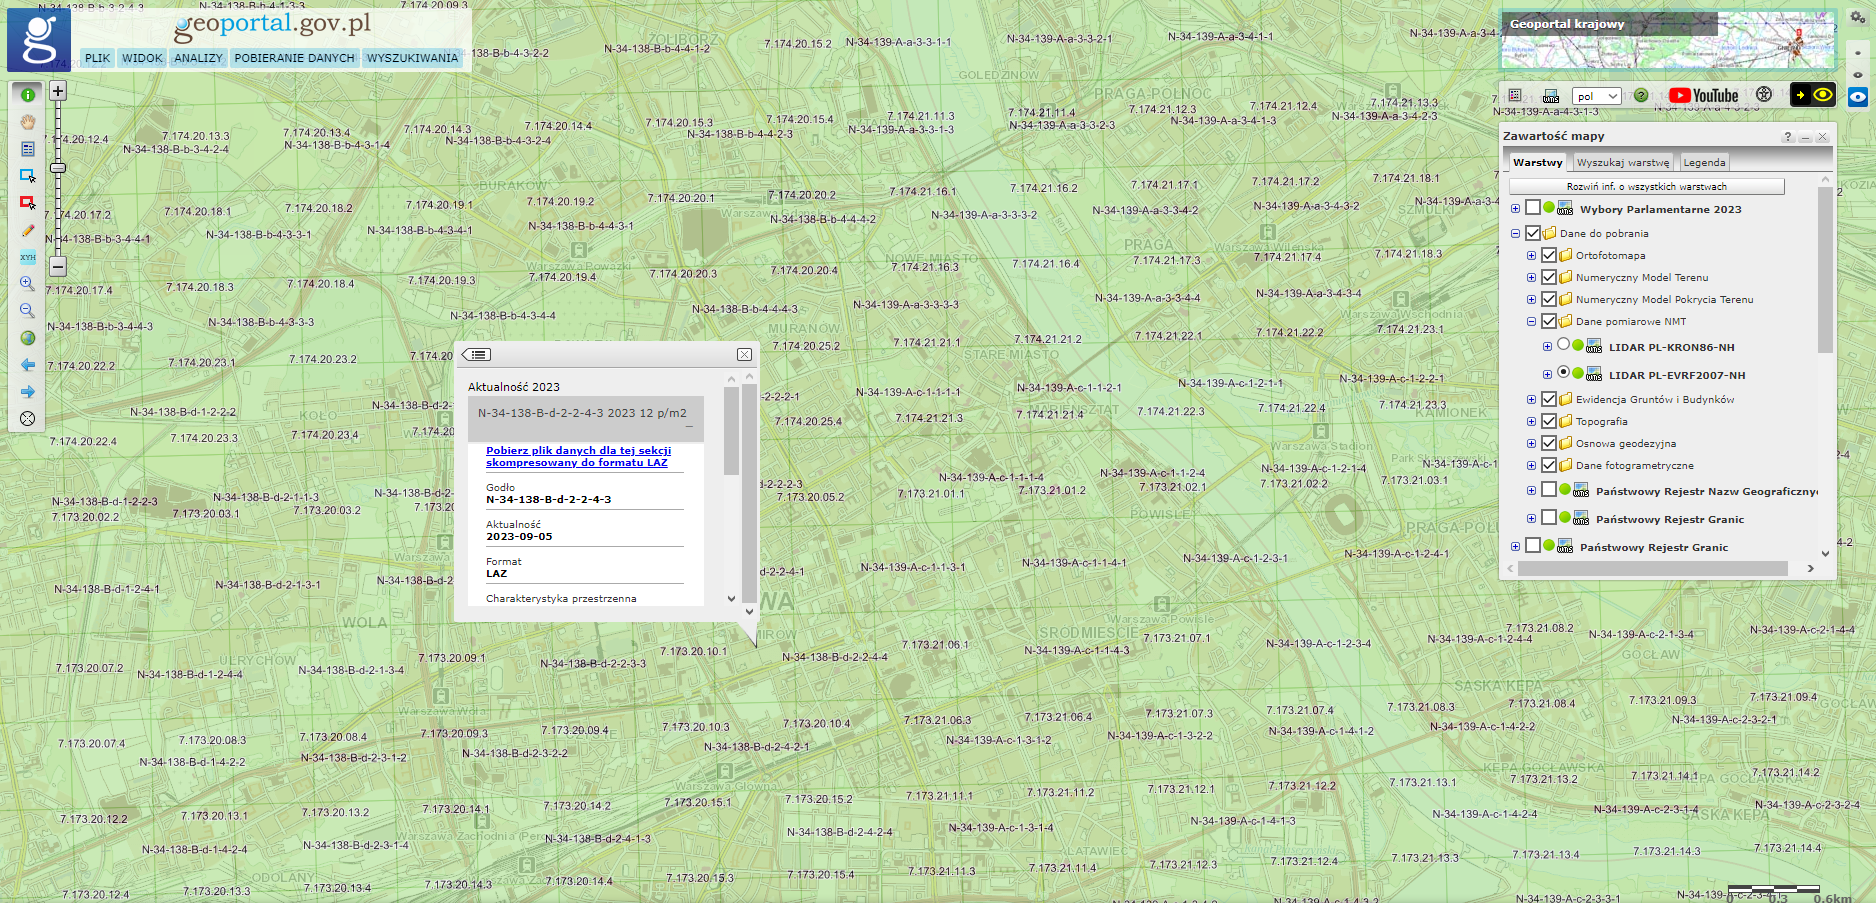
\includegraphics[width=\textwidth]{ISOK5.png}
	\caption{Then choose the newest version (usually the highest one) and use the link to download .laz file. Repeat this and previous step for every tile that covers your area of interest.}
	\label{fig:38}
\end{figure}

\begin{figure}[H]
	\centering
	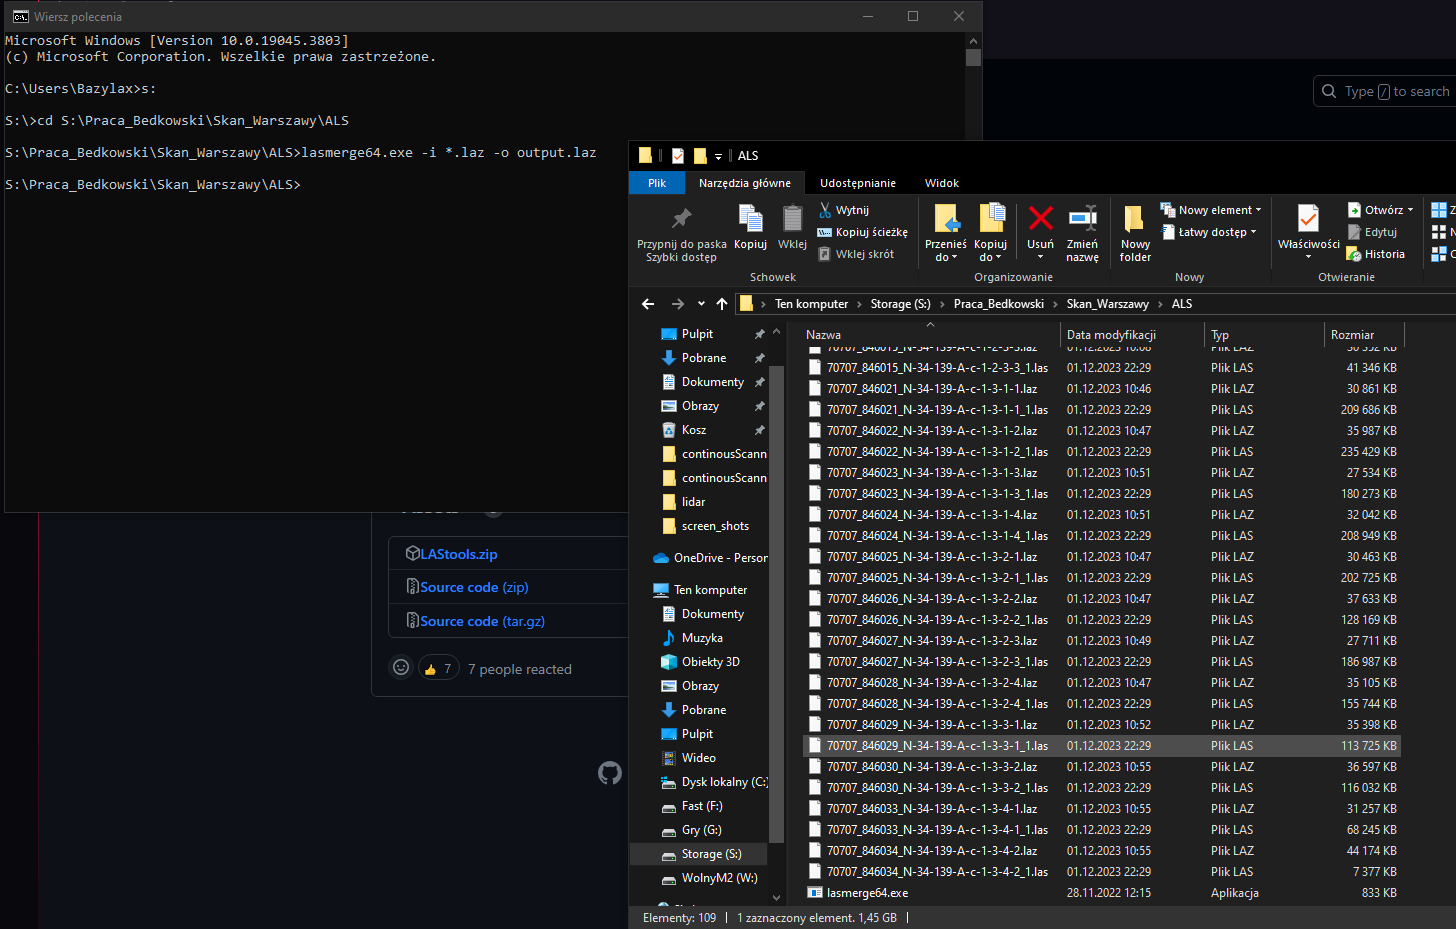
\includegraphics[width=\textwidth]{ISOK6.png}
	\caption{If merging of downloaded tiles is needed, I recommend using LAStools software. Download LAStools.zip from release page (\url{https://github.com/LAStools/LAStools/releases}). From folder bin/ extract lasmerge64.exe and put it in the folder where tile .laz files are stored. Open windows command prompt, move to directory with .laz files and write command: 
		\textit{lasmerge64.exe -i *.laz -o <your output .laz file name>.laz}}
	\label{fig:39}
\end{figure}

\begin{figure}[H]
	\centering
	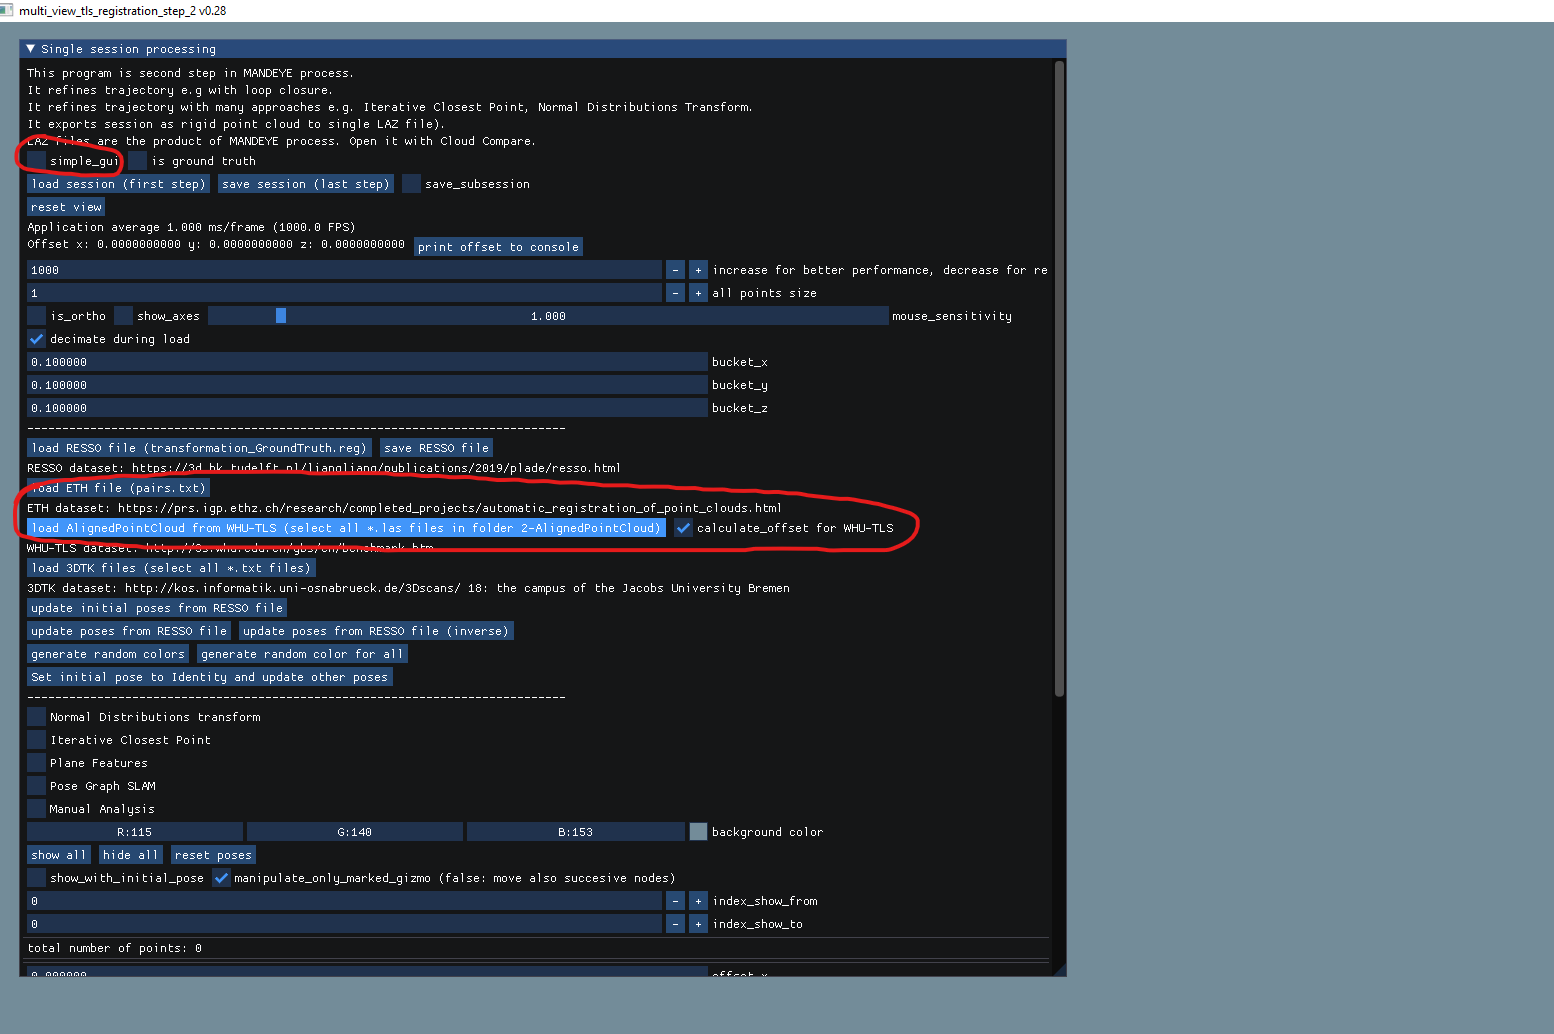
\includegraphics[width=\textwidth]{ISOK7.png}
	\caption{Open step 2 of this manual (\ref{fig:10}), unmatch simple gui, select calculate offset and load WHU-TLS data (many laz./las. files may be chosen).}
	\label{fig:40}
\end{figure}

\begin{figure}[H]
	\centering
	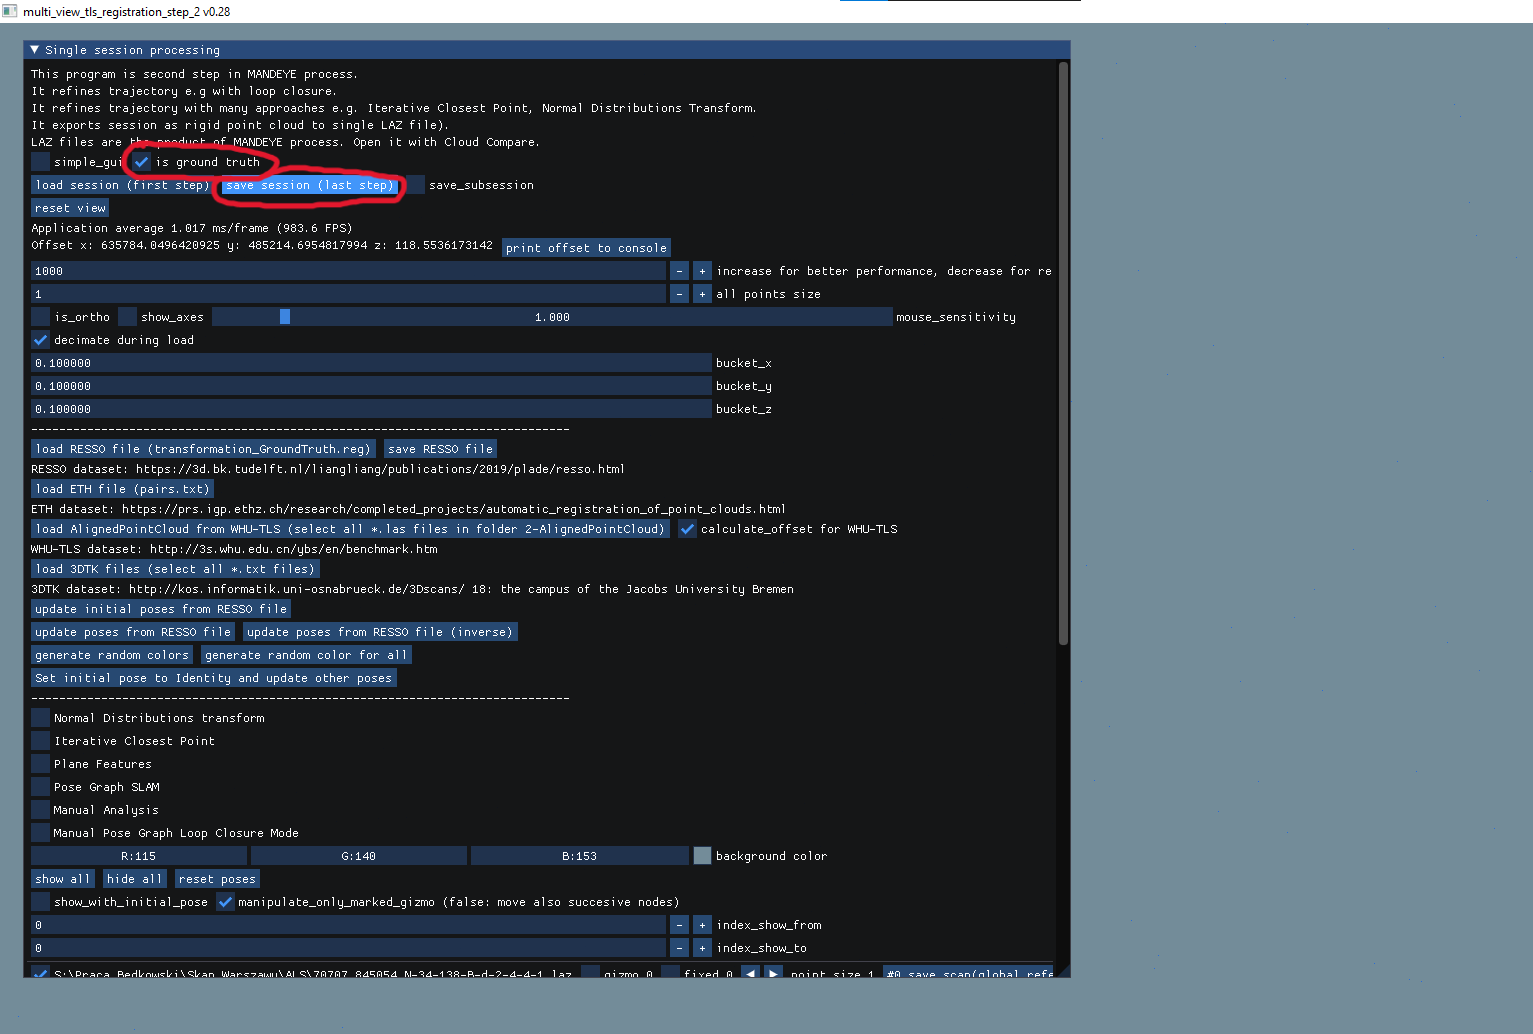
\includegraphics[width=\textwidth]{ISOK8.png}
	\caption{After loading scans successfully check ground truth option and save session as new .json file that contains all loaded scans. Now these scans may be loaded to serve as ground truth session that other scans can be aligned to.}
	\label{fig:41}
\end{figure}